%
% T�TULO DEL CAP�TULO
%
\chapter[ToView]{
	ToView
	\label{chapter_6}
}

ToView is how we named the visualizer that uses PCM under the hood, it was also implemented using C{}\verb!++!, OpenGL for visualization purposes and QT \cite{QT} for the user interface. All of these choices will be explained in the rest of the chapter.

\section[Design]{Design}

The visualizer has been implemented using \textbf{OpenGL 4.3} and \textbf{QT 5.3}. These two technologies were chosen so that the compatibility with multiple platforms was kept. Either OpenGL or QT are compatible with Windows, Linux and MacOS X.

On one hand, OpenGL is an API that allows an application to access and control the graphical system of the machine in which it is being executed. It could be a workstation with a high performance graphics card or a common desktop computer, a video-games console, etc.  

On the other hand, QT is a multi-platform graphical application creation framework. QT is open-source software that has been used and improved since it was created. It fits perfectly with our project since is C{}\verb!++! based. 

QT is used in more than 70 industries, by leading companies in their markets. QT is intuitive, has a suite for the design of interfaces called \textit{QT Designer} and plugins for the major development IDEs like Visual Studio.   

The compilers used as mentioned before are: Visual C{}\verb!++! in Windows systems, GCC in Linux and Clang in MacOS X.

\subsection[GUI]{Graphical User Interface}

\begin{figure}[h]
	\centering
	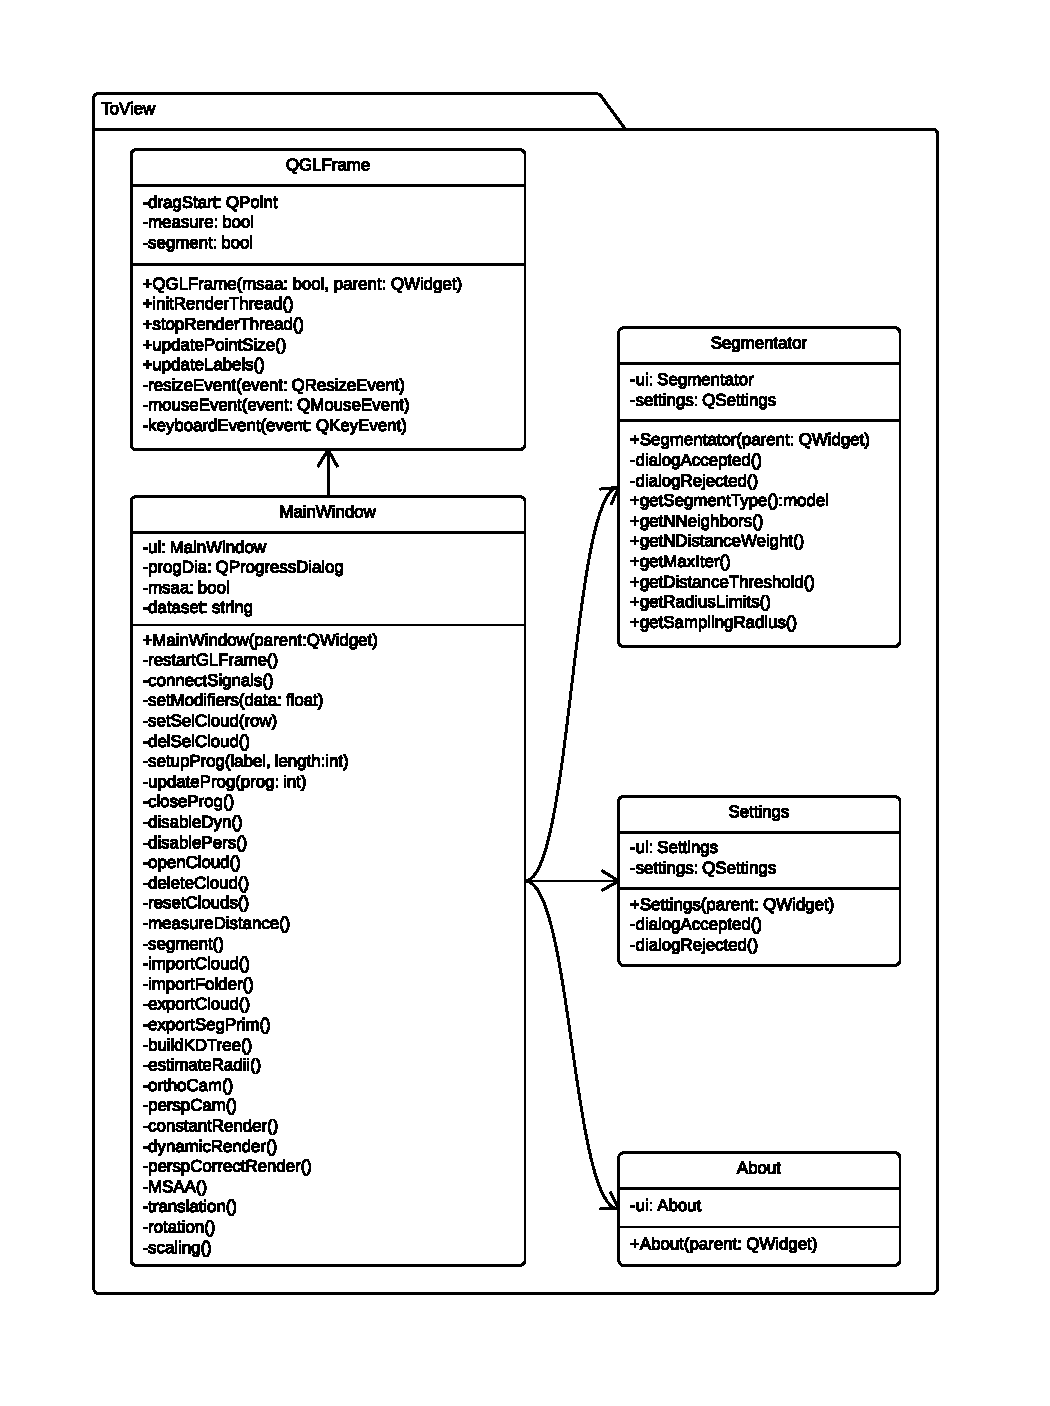
\includegraphics[scale=0.6]{figures/GUI.pdf}
	\caption[User interface class diagram]{
		Class diagram of the user interface of ToView.
	}
	\label{GUI}
\end{figure}

In the \autoref{GUI}, one of the main classes is \textbf{MainWindow}. This class gives the user access to all the functionality of the visualizer, it will serve as the name implies, as the main window in the interface. This class will centralize all the functionality and access to secondary dialogs, as well as communicate with the OpenGL context and render thread. 

The OpenGL context is represented in the interface by the class \textbf{QGLFrame}, that is in charge of creating the corresponding OpenGL context, render thread and displaying each frame rendered. This class will also handle all the keyboard and mouse events.  

The \textbf{Segmentator} class, is a sub-dialog that will let the user input the parameters for the segmentation of primitives in the clouds. All of the choices are saved using the \textbf{Qsettings} class. This QT class simplifies the process of managing settings in an application, eliminating the need for custom configuration files. 

Furthermore, \textbf{Settings} is another sub-dialog that allows the user to configure several visualizer parameters. This dialog also relies on \textbf{QSettings} to store the settings permanently. 

Finally, \textbf{About} is just another sub-dialog that shows information about the software (version, authors, etc.). 

\subsection[Render thread]{Render thread}

\begin{figure}[h]
	\centering
	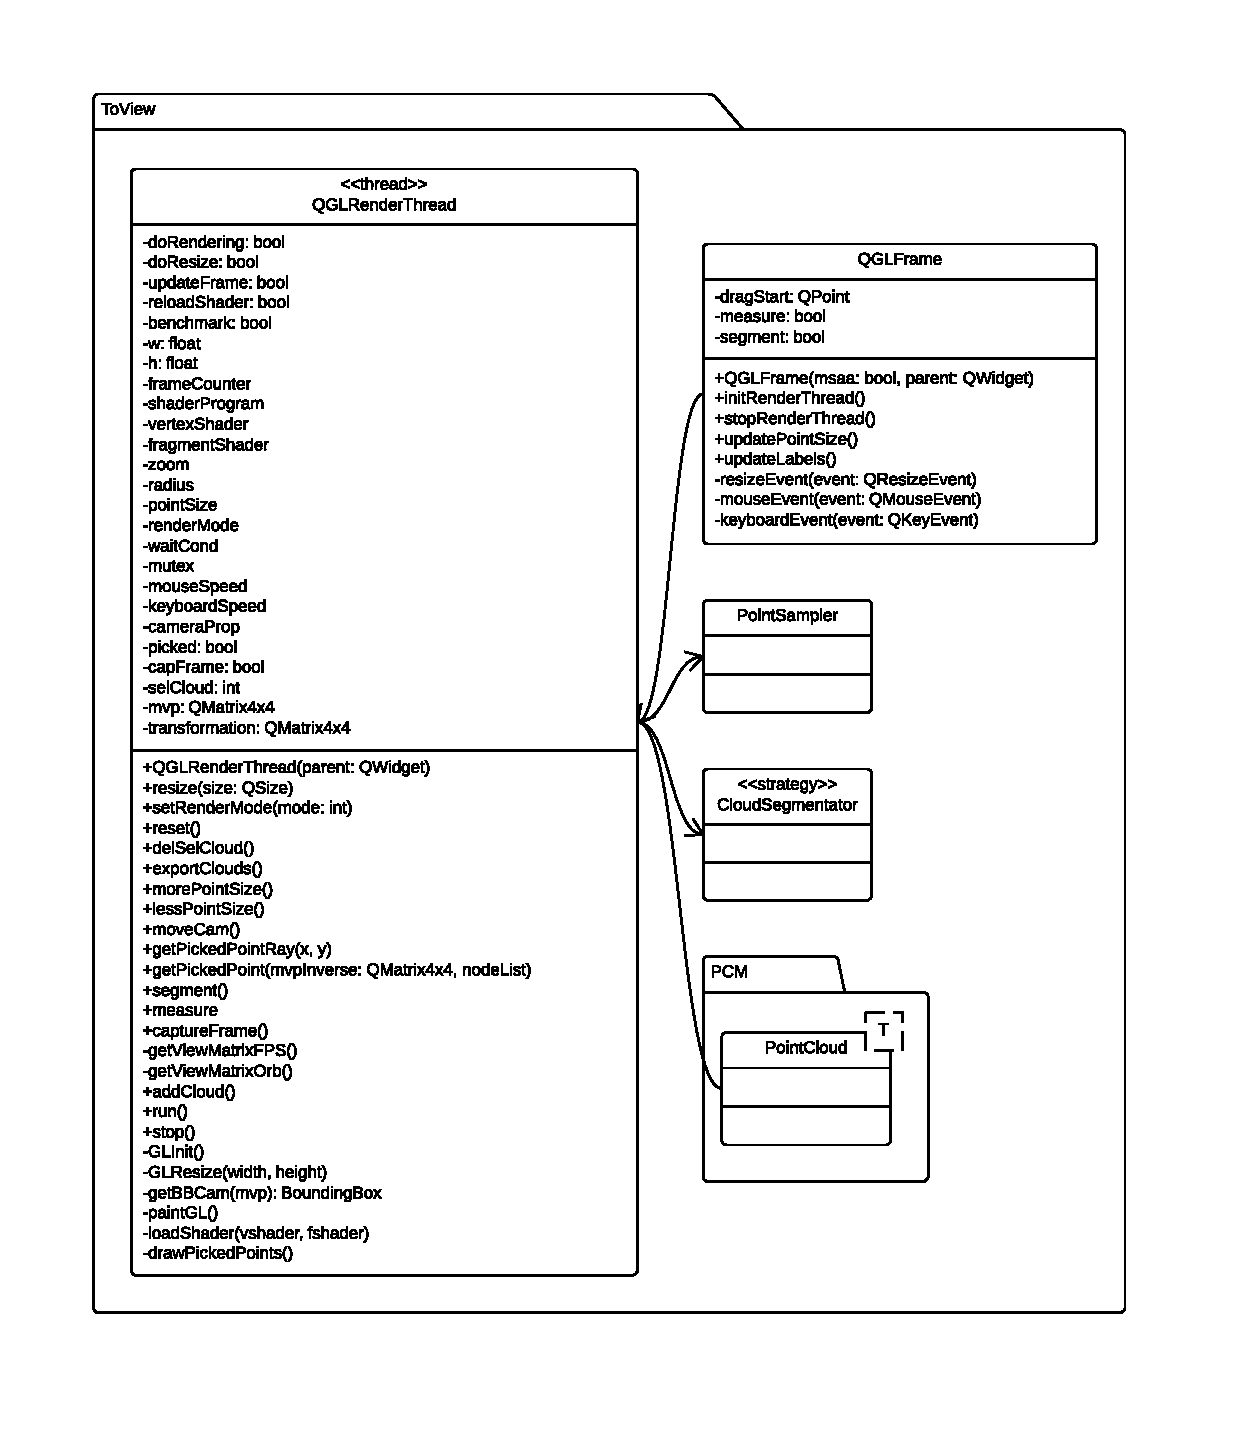
\includegraphics[scale=0.6]{figures/render_thread.pdf}
	\caption[Render thread class diagram]{
		Class diagram of the render thread and its related classes.
	}
	\label{render_thread}
\end{figure}

As we can observe in \autoref{render_thread}, \textbf{QGLRenderThread} is a extremely complex class, that as its name hints, represents a render thread. This class will be in charge of initializing OpenGL, loading shaders, rendering, calculating the camera parameters, etc.

The thread is created by \textbf{QGLFrame}, next the OpenGL context will be transferred to that thread so that the rendering can begin. Rendering is done in a different thread than the GUI, so that the latter will still be responsive even in the most demanding cases. 

Because of this, the communication between the render thread and the GUI will make use of QT \textit{signals} and \textit{slots}\footnote{Language tool introduced in QT for communication between objects, which allows the implementation of the Observer pattern. The concept is that GUI widgets can send signals containing event information, which can be received by other objects using special functions known as slots.}. With these tools, the communication between the different threads will be robust and simpler. Since the render thread could also be used from multiple threads, we will also use a \textit{mutex} to secure concurrent accesses.

To access the cloud information in PCM, the external interface \textbf{PointCloud} is used. \textbf{PointCloud} will provide the necessary information to render the desired clouds; like node lists, point data, memory hierarchy management, etc.      

\subsection[Segmentation]{Segmentation}

\begin{figure}[h]
	\centering
	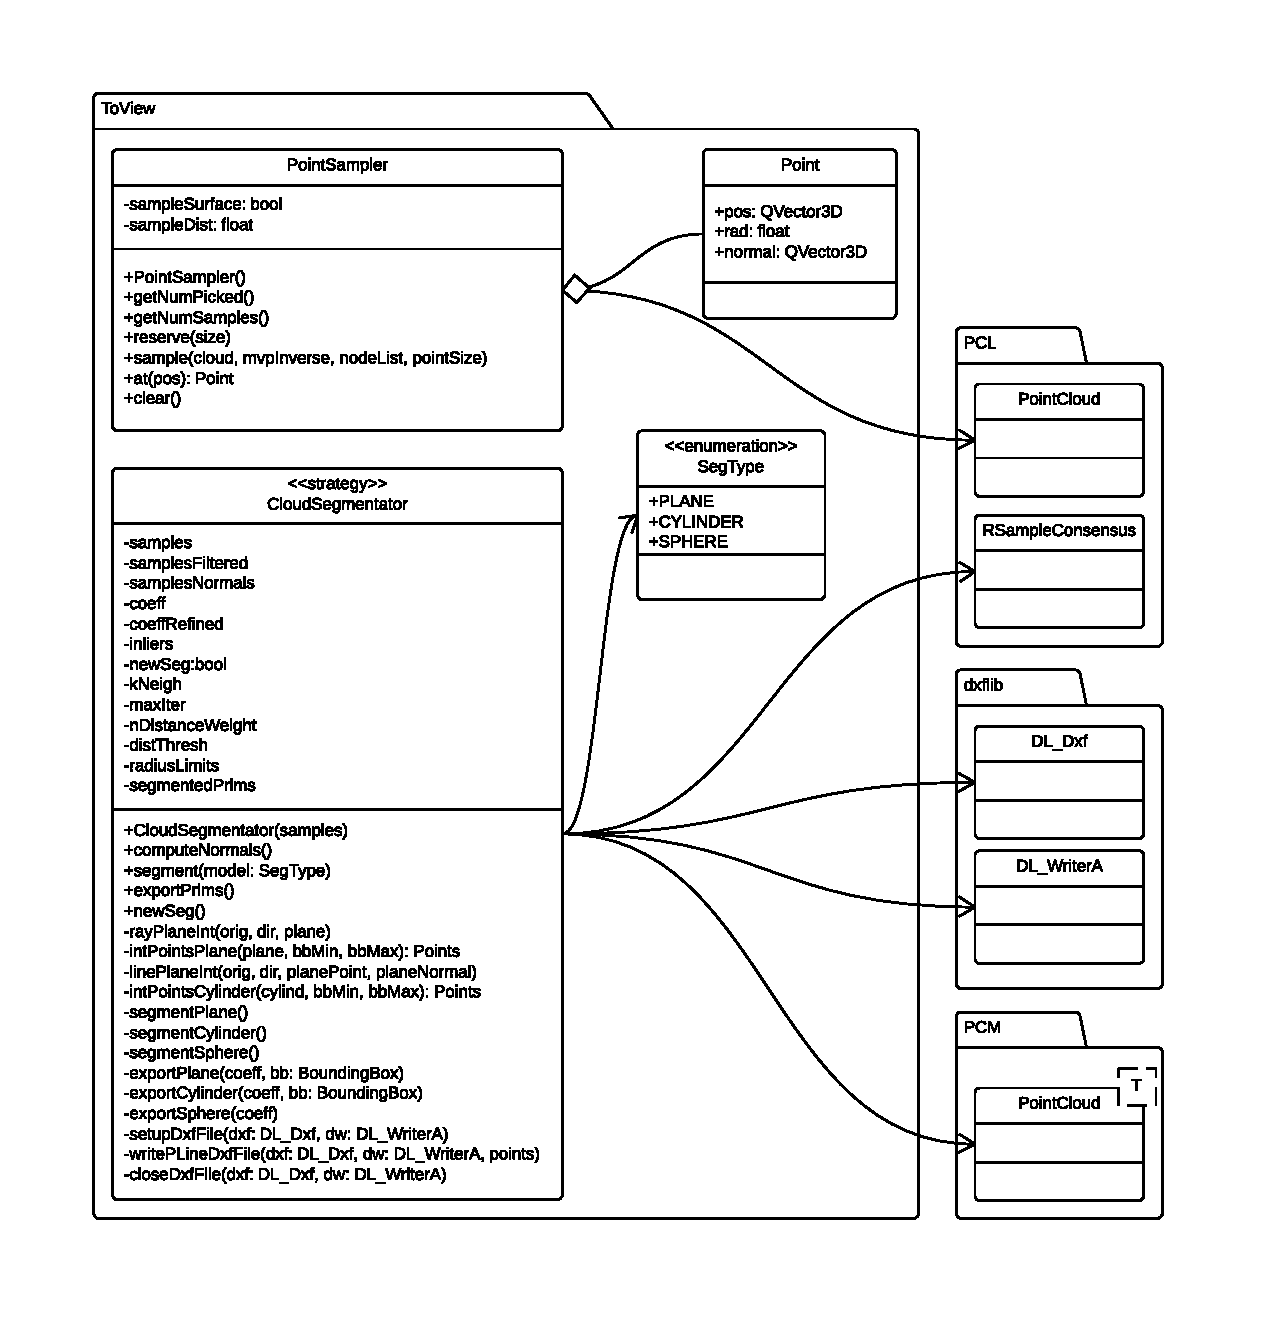
\includegraphics[scale=0.6]{figures/segmentation.pdf}
	\caption[Segmentation class diagram]{
		Class diagram of the classes related to segmentation.
	}
	\label{segmentation_class}
\end{figure}

In \autoref{segmentation_class}, the classes related to the segmentation process are detailed. One of the most significant classes is \textbf{PointSampler}, this will be the class that samples the corresponding point cloud and then converts the data so that it is compatible with PCL. It also is capable of picking individual points for distance measurements, and storing them in a similar fashion to a STL vector for quick access.   

Next, the most important class will be briefly explained. \textbf{CloudSegmentator} uses the information obtained by \textbf{PointSampler} to segment three types of primitives, \textit{planes}, \textit{cylinders} and \textit{spheres}. But this is not all the functionality that this class provides, it is also capable of exporting these primitives to an AutoCAD compatible format. 

To achieve these objectives, this class uses the \textbf{RSampleConsensus} class for primitive fitting and \textbf{DL\_Dxf} for \textit{DXF}\footnote{\textit{Drawing Exchange Format} is a CAD data file format developed by Autodesk for enabling data interoperability between AutoCAD and other programs.} exporting. Since there is not a good way to export cylinders and spheres in the DXF format, the segmentator will also support exporting these primitives as \textit{SCR}\footnote{\textit{Script Files} are simply a list of AutoCAD commands.} files.

Since some of the primitives need normals for the segmentation process, \textbf{CloudSegmentator} also includes the capability to estimate them. The pattern \textit{Strategy} was used for the design of this class so that adding primitives in the future will be easy. 

\section[Functionality]{Functionality}

The need for a robust tool to complement PCM was quickly noticed when using PCM's basic visualizer. This tool was enough for testing but left a lot to be desired, even when multiple clouds were not rendered onscreen and no advanced operations were performed on them. 

Moreover, the rendering code was written with the help of an open source scene graph called OSG\footnote{Open Scene Graph}. This was also an inconvenient because of the massive nature of the clouds that this software is designed to deal with. Heavy optimization would have to be performed and complete access to OpenGL rendering code was needed.

\begin{figure}[h]
	\centering
	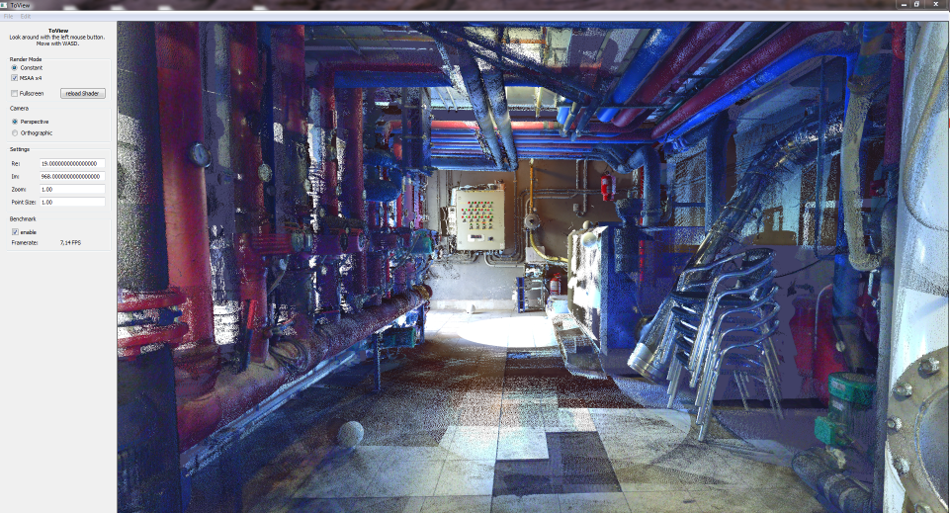
\includegraphics[scale=0.6]{figures/tovi_screen.png}
	\caption[Early ToView screenshot]{
		Screenshot showing an early version of ToView.
	}
	\label{early_toview}
\end{figure}

Furthermore, almost all of PCM's functionality was only accessible through multiple command line tools. When trying to integrate this software in engineering workflows, this was a big limitation.

If PCM was to be adopted by non-technical users, a GUI and more interactivity were essential. This is where ToView came to the rescue (see \autoref{early_toview}), with multiple cloud support, a GUI, advanced rendering, distance measuring capabilities, object detection, etc. All the functionality that ToView brings to the table will be exposed in the following subsections.

\subsection[Render modes]{Render modes}

In light of the need for high quality point based rendering, but also trying to keep versatility, three rendering modes are supported in ToView:

\begin{itemize}
	\item \textbf{Constant:} Most basic type of point-based rendering, it does not require point normals or radii.
	\item \textbf{Dynamic:} Almost the same as the previous mode, but requires point radii to reduce clipping and increase rendering quality and performance.
	\item \textbf{Perspective accurate:} Most advanced type of rendering, requires point normals and radii. This rendering mode yields high quality renders but at a greater computational cost.
\end{itemize}

\begin{figure}[h]
	\centering
	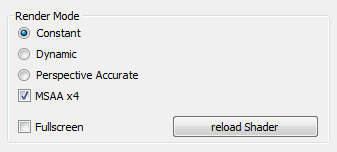
\includegraphics[scale=0.9]{figures/render_modes.png}
	\caption[Render modes]{
		Screenshot showing all of the available render modes in ToView's interface.
	}
	\label{render_modes}
\end{figure}

As we can see in \autoref{render_modes}, more parameters like anti-aliasing or full-screen rendering are also exposed through the GUI. Anti-aliasing will play a huge role in high quality rendering as it increases image quality dramatically.

All of these rendering modes and a complementary technique that was not exposed to the user in ToView, but was also implemented for testing, will be explained in depth in \autoref{chapter_7}.

\subsection[Camera types]{Camera types}

Since camera only one camera type was present in the old visualizer, two types of camera paradigms were implemented:

\begin{itemize}
	\item \textbf{First-person camera:} Type of camera that imitates how movement is implemented in video games. This camera is ideal for virtual tours of the scenes, or working with really big scenes with multiple objects.
	\item \textbf{Orbital:} This camera model emulates cameras in modeling software (Blender, AutoCAD, etc.). This camera type is optimal for working with single objects and an orthographic projection.
\end{itemize}

Furthermore, because of the engineering nature of our software, a perspective camera may not be the optimal choice. This is the reason why two types of projection are available for the user:

\begin{itemize}
	\item \textbf{Perspective:} Projection model that reflects how the human eye perceives scenes, objects in the distance appear smaller than objects close by. This projection type is useful when moving through a city or interior datasets. 
	\item \textbf{Ortographic:} This projection type ignores the aforementioned effect so that to-scale modeling can occur. This projection model is useful when working with single objects or when we need to see parallel lines as parallel in the final image.
\end{itemize}

All of these camera types are controlled using the keyboard and mouse, trying to make it as easy as possible for the end user. The math and implementation details behind these cameras are explained in \autoref{camera_model}. The options are exposed to the user through a convenient menu in the interface and do not require restarting the application to be applied (see \autoref{camera_types}).

\begin{figure}[h]
	\centering
	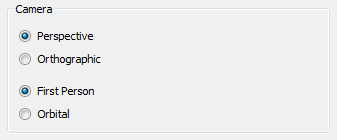
\includegraphics[scale=0.9]{figures/camera_types.png}
	\caption[Camera options]{
		Screenshot showing all of the available camera options in ToView's interface.
	}
	\label{camera_types}
\end{figure}

\subsection[Preprocessing]{Preprocessing}

As mentioned before, scanners sometimes output clouds that may not be optimal for the task at hand. As a consequence, some preprocessing can be needed. ToView offers its users several operations:

\begin{itemize}
	\item \textbf{Voxel grid filter:} Downsampling filter, useful to thin dense point clouds or keep the cloud density uniform. 
	\item \textbf{Statistical outlier removal:} Noise removal filter, it can be used to remove outliers or noise present in the clouds.
	\item \textbf{Radii estimation:} Necessary process if the end user wants to use the two advanced rendering modes. It estimates the value of the point radii.
	\item \textbf{K-d tree building:} Essential process for the visualization of the point clouds. Without a spatial acceleration structure, the clouds would be too big to render or perform any operation.
\end{itemize}

The preprocessing filters are further explained in \autoref{chapter_9}. All of these point cloud operations are exposed to the user through the tools menu in the interface(see \autoref{tools_menu}).

\begin{figure}[h]
	\centering
	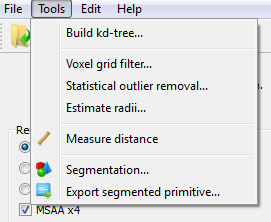
\includegraphics[scale=0.7]{figures/tools.png}
	\caption[Tools menu]{
		Screenshot showing all of the available point cloud tools in ToView's interface.
	}
	\label{tools_menu}
\end{figure}

\subsection[Cloud interaction]{Cloud interaction}

One of the main drawbacks of having a simple visualizer without a GUI was the inability to integrate multiple point clouds, and perform modifications on the clouds (see \autoref{mult_clouds}). 

\begin{figure}[h]
	\centering
	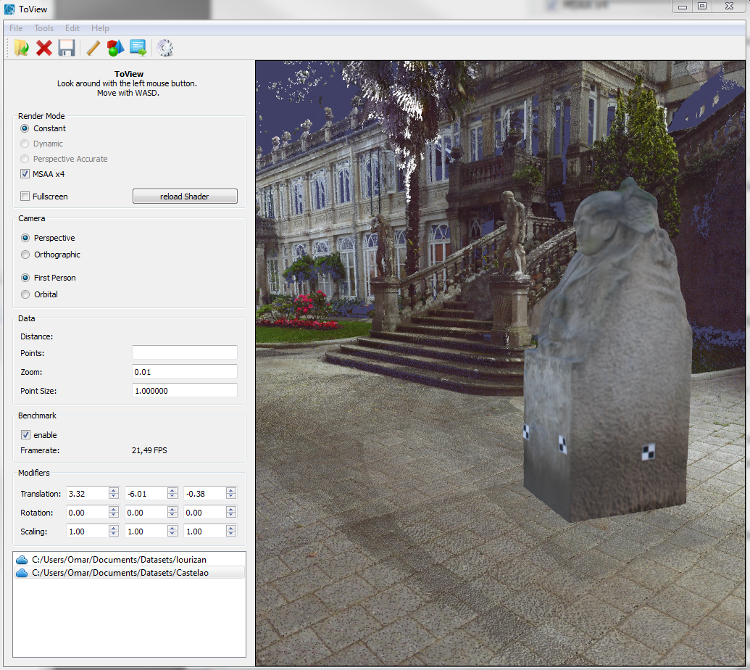
\includegraphics[scale=0.495]{figures/mult_clouds_int.png}
	\caption[Multiple point cloud integration]{
		Two clouds (a park and a statue) integrated using ToView.
	}
	\label{mult_clouds}
\end{figure}

ToView offers multiple possibilities on this front:

\begin{itemize}
	\item \textbf{Point cloud transformation:} Each cloud can be transformed to the user's liking. 
	\begin{itemize}
		\item \textbf{Translation:} The cloud can be moved through space.
		\item \textbf{Rotation:} The cloud can be rotated.
		\item \textbf{Scaling:} The cloud can be transformed to be bigger or smaller.
	\end{itemize}
	\item \textbf{Multiple point cloud integration:} The user can transform multiple clouds at the same time. This allows the integration of multiple point clouds, correcting positioning errors, wrong coordinate systems, etc.
	\item \textbf{Cloud selector:} Select a cloud to transform, eliminate or perform any operation in an easy way through the interface.
\end{itemize}

The aforementioned features are exposed through the interface in a panel in the interface (see \autoref{cloud_modifiers}). All of these features work in real-time, allowing the user to see the changes made reflected instantly. Clouds can also be added or removed in real-time according to the user's needs.   

\begin{figure}[h]
	\centering
	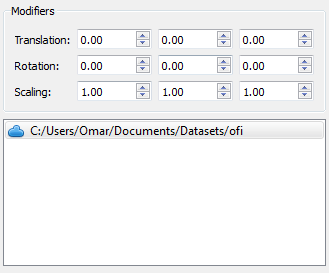
\includegraphics[scale=0.7]{figures/cloud_modif.png}
	\caption[Cloud interaction]{
		Screenshot showing the cloud interaction menu in ToView's interface.
	}
	\label{cloud_modifiers}
\end{figure}

\subsection[Point picking]{Point picking}

In order to be able to measure distances or segment primitives interactively in the clouds, the visualizer has to be capable of finding the correct point that the user desires in the clouds. This action is called point picking, and is performed in real-time by the visualizer. 

To achieve this, the first step is getting the position the user has clicked in the window. This is done using QT's API and returns two values, the $x$ and $y$ coordinates.

Secondly, the coordinates are transformed so that we have the coordinates of a ray corresponding to that pixel in NDC. The ray origin can be obtained with the following equation:

\begin{equation} \mathbf{r_{start}} = ((x/w - 0.5) * 2, (y/h - 0.5) * 2, 0) \end{equation} 

Being $w$ the width of the window and $h$ the height. The ray end can be obtained with the equation that follows:

\begin{equation} \mathbf{r_{end}} = ((x/w - 0.5) * 2, (y/h - 0.5) * 2, 1) \end{equation} 

Once we have the ray in NDC space, we need to transform it to world space. The operation needed to get the ray in world space is just a matrix multiplication:

\begin{equation} \mathbf{r_{world}} = \textbf{\textit{MVP}}^{-1} \cdot \mathbf{r_{ndc}} \end{equation}

Finally, after the ray in world coordinates is obtained, it is just a matter of obtaining the points that intersect with the ray and then return the closest to the viewpoint.

To use this functionality, the user will just have to right-click the mouse, and the visualizer will take care of all of the steps internally (see \autoref{picked_point}).

\begin{figure}[h]
	\centering
	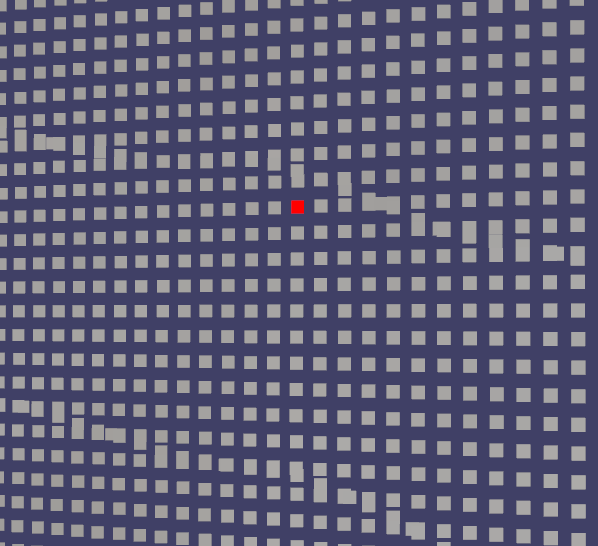
\includegraphics[scale=0.6]{figures/picked_point.png}
	\caption[Point picking example]{
		Screenshot showing the picked point in a cloud in red.
	}
	\label{picked_point}
\end{figure}

\subsection[Distance measurements]{Distance measurements}

A typical operation in a point cloud for engineers is measuring distances. The surveyor nowadays, does not have to go back to the field each time a new measurement is needed. With point clouds, the laser scanner will register data of every surrounding surface and all of the information will be stored in the point cloud for later use. 

Therefore, once we have the ability to select two or more points, we will have the possibility of obtaining measurements. The accuracy of the measurements, will depend on the precision of the scanner (the scanner that we are using has millimeter precision). Having the points $\mathbf{p_{1}}$ and $\mathbf{p_{2}}$, the distance is obtained with the following equation:

 \begin{equation} D = \lVert \mathbf{p_{1}} - \mathbf{p_{2}} \rVert \end{equation}
 
The user just needs to click the distance measurement option in the tools menu (see \autoref{tools_menu}) and then select two points in the cloud. The measurement will be performed in real-time and the result displayed in the interface (see \autoref{dist_measurement}).

\begin{figure}[h]
	\centering
	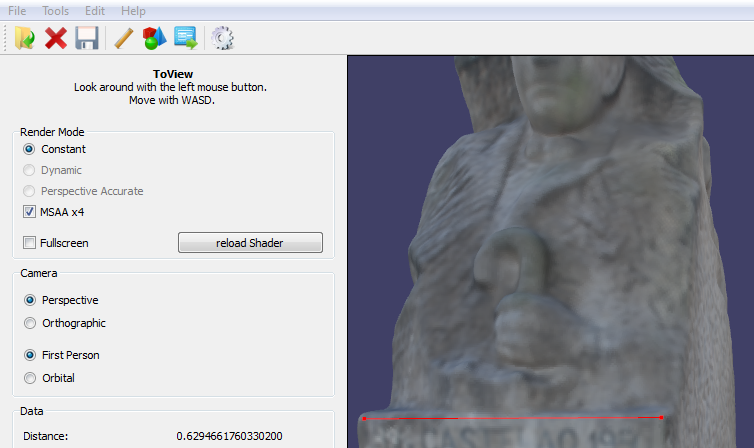
\includegraphics[scale=0.7]{figures/dist_measurement.png}
	\caption[Distance measurement example]{
		Screenshot showing a distance measured in a point cloud.
	}
	\label{dist_measurement}
\end{figure}

\subsection[Primitive segmentation]{Primitive segmentation}

Another feature widely requested by civil engineers, is the estimation of parametric primitives from the point cloud. To better explain the usefulness of this feature, the reader may think of a pipe. If we wanted to select each point to extract the cloud representing the pipe or create an CAD representation of the object, how would we go about it? This is not a trivial problem, and even less when dealing with massive point clouds.

To solve this problem, in ToView we have designed a semi-automatic way of segmenting objects. The steps involved in this process are:

\begin{enumerate}
	\item The user selects a point in the cloud. 
	\item The visualizer samples the surrounding area.
	\item Estimates the necessary features.
	\item Uses RANSAC to estimate the chosen primitive.
	\item Displays the result to the user.
\end{enumerate}

Due to the limited time available to implement an ambitious project as this one, PCL was integrated with ToView to make use of the implemented RANSAC classes available in PCL. Thanks to this we have been able to test advanced RANSAC implementations and employ more time investigating and making the visualizer more robust. 

\begin{figure}[h]
	\centering
	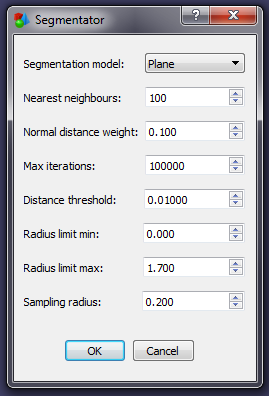
\includegraphics[scale=0.7]{figures/segmentation_dialog.png}
	\caption[Segmentation dialog]{
		Screenshot showing the segmentation options available.
	}
	\label{seg_dia}
\end{figure}

PCL is a widely used point cloud library, with lots of features not only limited to RANSAC implementations. In the future it will be interesting to integrate PCL further, for normal estimation, advanced segmentation, etc.

ToView is capable of estimating planes, cylinders and spheres. The process also allows the user to further refine the primitives selecting more points after the initial estimation (see \autoref{estimated_cyl}).

\begin{figure}[h]
	\centering
	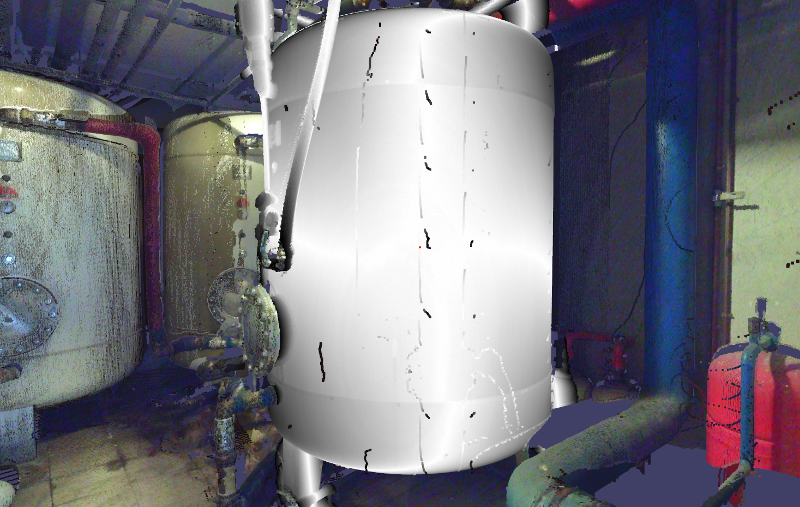
\includegraphics[scale=0.7]{figures/seg_cyl.png}
	\caption[Segmented cylinder]{
		Screenshot showing a segmented cylinder.
	}
	\label{estimated_cyl}
\end{figure}

This estimation is also performed in real-time and is easily accessible from the GUI. When the user clicks on the option to segment primitive (see \autoref{tools_menu}), a new dialog will appear that will let the user fine tune the segmentation options (see \autoref{seg_dia}). The process is really intuitive for the user, as it is only needed to select a point of the object that needs to be segmented.

All of the theory behind primitive segmentation will be explained in depth in \autoref{chapter_8}.

\subsection[Primitive exportation]{Primitive exportation}

In order to use the estimated parametric primitives, we will have to export them in a format that other software can read. Therefore, \textit{DXF}, a standard CAD exchange format was chosen for planes and \textit{SCR} an AutoCAD scripting format for more complex primitives like cylinders or spheres. 

To create the exported DXF file, we have used dxflib \cite{dxflib}, an open source library for the manipulation of DXF files.

In order to highlight and export these primitives, some previous steps are needed. Namely, calculating the point-primitive distance and bounding the primitives. These two steps are extensively explained in \autoref{chapter_8}. 

ToView supports the estimation of any number of primitives and the exportation in one step of all of them. The user just has to select the option export segmented primitive in the tools menu (see \autoref{tools_menu}).

\begin{figure}[h]
	\centering
	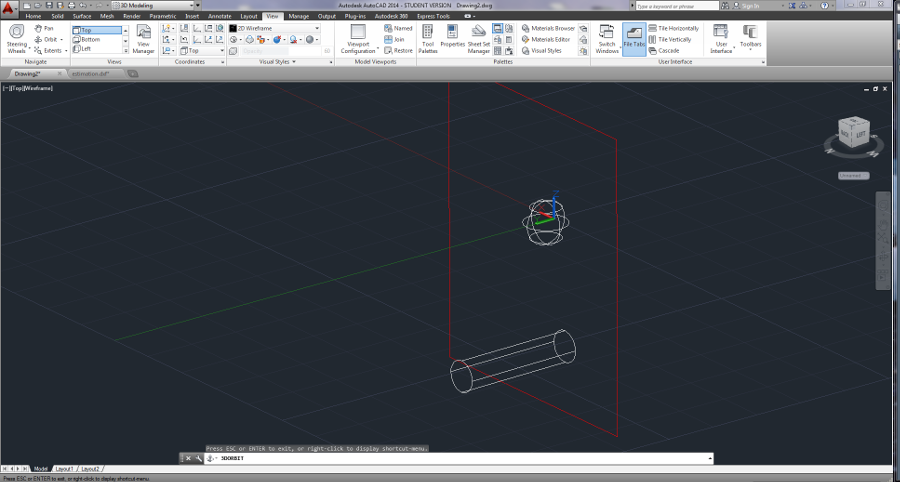
\includegraphics[scale=0.55]{figures/autocad.png}
	\caption[Segmented primitives in AutoCAD]{
		A segmented plane, cylinder and sphere opened in autocad.
	}
	\label{autocad}
\end{figure}

This feature has the potential to substantially reduce the time needed to create CAD models of rooms, pipes, etc. (see \autoref{autocad}). It also has the potential to clean clouds faster, the surveyor just needs to click on a point to select the complete object (in contrast to manually selecting all the points), and then choose what to do with it. 

\section[Results]{\label{sec:tov_results}Results}

Again, two different computers were used for testing. The first, \textbf{Computer 3} has the following specs:

\begin{itemize}
	\item Intel Core i7-2600K CPU (4 cores, 8 threads)
	\item NVIDIA GTX 680 graphics card
	\item 8 GB of 1600 MHz DDR3 RAM
	\item WD Caviar Black HDD
\end{itemize} 

The second, \textbf{Laptop 1} has the following specifications:

\begin{itemize}
	\item Intel Core i7-3632QM CPU (4 cores, 8 threads)
	\item NVIDIA GT 720M graphics card
	\item 16 GB of 1333 MHz DDR3L RAM
	\item SSHD
\end{itemize} 

The operating systems used to run the tests were: 

\begin{itemize}
	\item Windows 7 x64 with the VC{}\verb!++! v110 compiler
	\item Ubuntu 14.04 x64 with the GCC 4.8 compiler
\end{itemize} 

The libraries used were:

\begin{itemize}
	\item QT 5.3
	\item OSG 3.0.1
	\item GLEW 1.10.0
	\item PCL 1.7.1
\end{itemize} 

The datasets that will be used for testing are described in \autoref{dataset_table}. The L1 cache size used in Computer 1 was 1500 MB, while in Laptop 1 was 512 MB. In addition, the L2 cache size used in Computer 1 was 4 GB and in Laptop 1 was 1 GB. The cache settings used are those recommended in \autoref{sec:res_pcm}

\begin{figure}[h]
	\centering
	\subfigure[Computer 3]{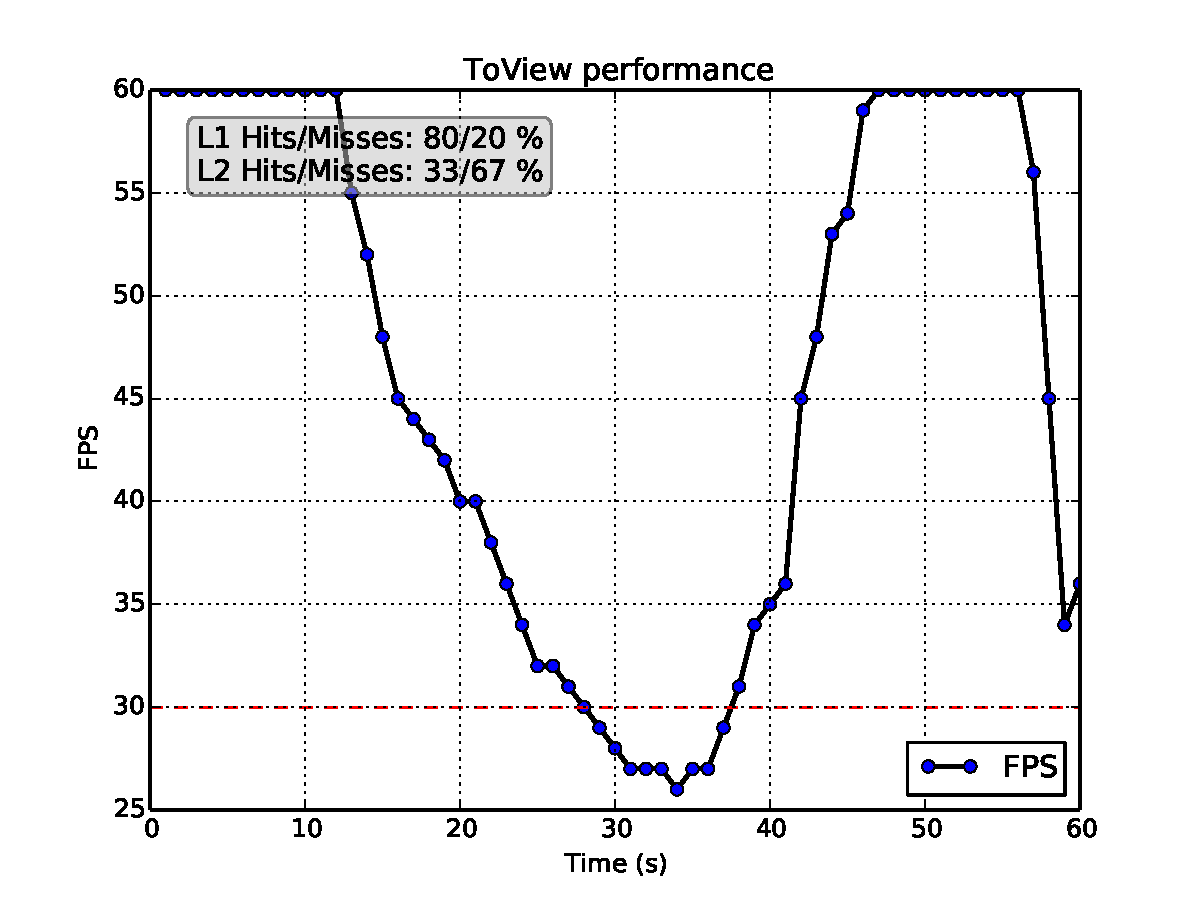
\includegraphics[width=0.49\textwidth]{figures/desktop_lour.pdf}}
	\subfigure[Laptop 1]{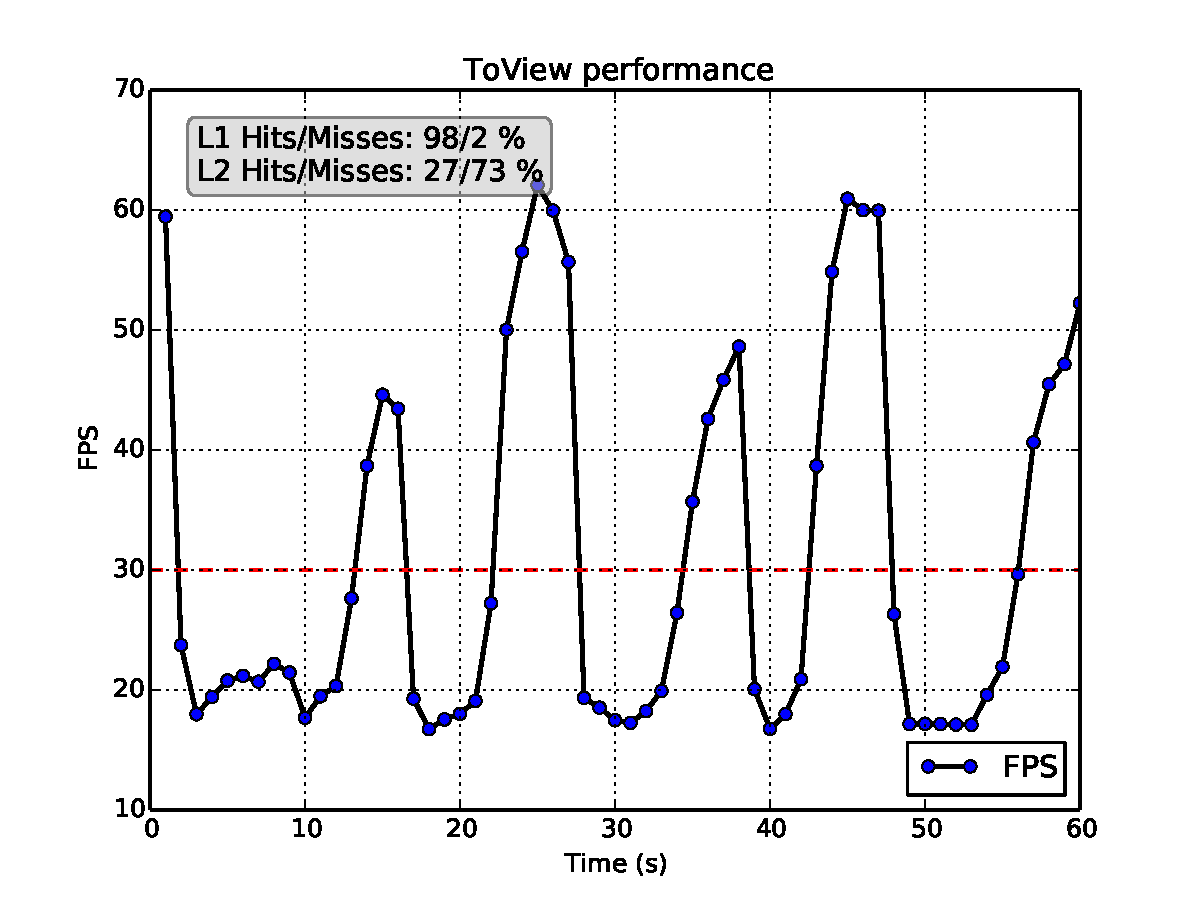
\includegraphics[width=0.49\textwidth]{figures/laptop_lour.pdf}}
	\caption[FPS obtained in Lourizan]{
		Graphs showing the FPS that ToView achieves in the Lourizan dataset.
	}
	\label{fps_lour}
\end{figure}

Since the smaller datasets tested (Castelao, Dorna, etc.) obtained 60 FPS in both computers, we will not present graphs with the results. The first truly taxing dataset tested was lourizan as can be seen on \autoref{fps_lour}.